\documentclass[11pt,a4paper]{report}
\usepackage[spanish,es-nodecimaldot]{babel}	% Utilizar español
\usepackage[utf8]{inputenc}					% Caracteres UTF-8
\usepackage{graphicx}						% Imagenes
\usepackage[hidelinks]{hyperref}			% Poner enlaces sin marcarlos en rojo
\usepackage{fancyhdr}						% Modificar encabezados y pies de pagina
\usepackage{float}							% Insertar figuras
\usepackage[textwidth=390pt]{geometry}		% Anchura de la pagina
\usepackage[nottoc]{tocbibind}				% Referencias (no incluir num pagina indice en Indice)
\usepackage{enumitem}						% Permitir enumerate con distintos simbolos
\usepackage[T1]{fontenc}					% Usar textsc en sections
\usepackage{amsmath}				% Símbolos matemáticos
\usepackage{listings}
\usepackage{color}

 
\definecolor{codegreen}{rgb}{0,0.6,0}
\definecolor{codegray}{rgb}{0.5,0.5,0.5}
\definecolor{codepurple}{rgb}{0.58,0,0.82}
\definecolor{backcolour}{rgb}{0.95,0.95,0.95}
 
\lstdefinestyle{mystyle}{
    backgroundcolor=\color{backcolour},   
    commentstyle=\color{codegreen},
    keywordstyle=\color{magenta},
    numberstyle=\tiny\color{codegray},
    stringstyle=\color{codepurple},
    basicstyle=\footnotesize,
    breakatwhitespace=false,         
    breaklines=true,                 
    captionpos=b,                    
    keepspaces=true,                 
    numbers=left,                    
    numbersep=5pt,                  
    showspaces=false,                
    showstringspaces=false,
    showtabs=false,                  
    tabsize=2
}
 
\lstset{style=mystyle, language=C++}

% Comando para poner el nombre de la asignatura
\newcommand{\asignatura}{Simulación de Sistemas}
\newcommand{\autor}{José María Sánchez Guerrero}
\newcommand{\titulo}{Práctica 3}
\newcommand{\subtitulo}{Modelos de Simulación Dinámicos y Discretos}

% Configuracion de encabezados y pies de pagina
\pagestyle{fancy}
\lhead{\autor{}}
\rhead{\asignatura{}}
\lfoot{Grado en Ingeniería Informática}
\cfoot{}
\rfoot{\thepage}
\renewcommand{\headrulewidth}{0.4pt}		% Linea cabeza de pagina
\renewcommand{\footrulewidth}{0.4pt}		% Linea pie de pagina

\begin{document}
\pagenumbering{gobble}

% Pagina de titulo
\begin{titlepage}

\begin{minipage}{\textwidth}

\centering

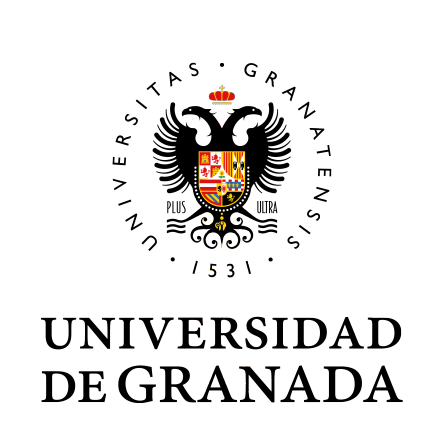
\includegraphics[scale=0.5]{img/ugr.png}\\

\textsc{\Large \asignatura{}\\[0.2cm]}
\textsc{GRADO EN INGENIERÍA INFORMÁTICA}\\[1cm]

\noindent\rule[-1ex]{\textwidth}{1pt}\\[1.5ex]
\textsc{{\Huge \titulo\\[0.5ex]}}
\textsc{{\Large \subtitulo\\}}
\noindent\rule[-1ex]{\textwidth}{2pt}\\[3.5ex]

\end{minipage}

\vspace{0.5cm}

\begin{minipage}{\textwidth}

\centering

\textbf{Autor}\\ {\autor{}}\\[2.5ex]
\textbf{Rama}\\ {Computación y Sistemas Inteligentes}\\[2.5ex]
\vspace{0.3cm}


\includegraphics[scale=0.3]{img/etsiit.jpeg}

\vspace{0.7cm}
\textsc{Escuela Técnica Superior de Ingenierías Informática y de Telecomunicación}\\
\vspace{1cm}
\textsc{Curso 2019-2020}
\end{minipage}
\end{titlepage}

\pagenumbering{arabic}
\tableofcontents
\thispagestyle{empty}				% No usar estilo en la pagina de indice

\newpage

\setlength{\parskip}{1em}

\chapter{Mi segundo modelo de simulación Discreto}

Nuestro modelo de simulación consistirá en un servidor que presta un determinado servicio a una serie de clientes, los cuales solicitarán dicho servicio
periódicamente. Cuando llega un cliente y el servidor no está ocupado, será atendido inmediatamente; en caso contrario, el cliente tendrá que esperar en
la cola. Cuando se completa un servicio, el servidor elegirá al siguiente en una forma FIFO.

Al empezar la simulación, no habrá clientes esperando y el servidor está libre. Utilizaremos el mismo generador exponencial tanto para el tiempo que tardarán
en llegar los clientes, como el tiempo que tardará el servidor en atender a cada uno.


\section{Simulación con incremento fijo de tiempo}

En esta simulación, vamos a tratar al tiempo incrementándolo de unidad en unidad. Para evitar problemas con el manejo del tiempo, tendremos que modificar
los generadores de datos para que nos devuelvan los valores redondeados al entero más próximo. Si obtenemos un valor igual a 0, devolveremos 1 en su lugar,
ya que el suceso generado quedaría en un tiempo anterior al actual, que generamos al incrementar en una unidad.

Este será nuestro código resultante, que nos servirá tanto para generar el tiempo de llegada del cliente como para generar el timepo del servicio (sólo
tendremos que modificar la variable $tlleg$ por $tserv$):
\newpage
\begin{lstlisting}
float generallegada(float tlleg){
	float u = random();         // o tambien rand() en lugar de random()
	u = ( u / (RAND_MAX+1.0) ); //RAND_MAX es una constante del sistema
	u = round( -tlleg * log(1-u) );

	if (u != 0)
		return u;
	else
		return 1.0;
}
\end{lstlisting}


Para la simulación vamos a emplear diferentes unidades de medida de tiempo (horas, minutos, segundos...) y con un número de clientes a atender bastante alto,
de unos 10.000, para que los resultados sean robustos. Este es el resultado que obtenemos:
\begin{table}[H]
\resizebox{\textwidth}{!}{%
\begin{tabular}{c|c|c|c|c}
\textbf{tiempo} & \textbf{tlleg} & \textbf{tserv} & \textbf{\% tiempo ocioso} & \textbf{Media clientes en cola} \\ \hline
horas           & 0.15           & 0.1            & 0.019994                  & 0.000000                        \\ \hline
medias horas    & 0.3            & 0.2            & 0.625621                  & 0.078153                        \\ \hline
cuartos de hora & 0.6            & 0.4            & 7.224885                  & 0.356633                        \\ \hline
minutos         & 9              & 6              & 31.501728                 & 1.647961                        \\ \hline
segundos        & 540            & 360            & 33.934223                 & 1.282934                        \\
\end{tabular}%
}
\end{table}

Como podemos ver, los porcentajes de tiempo ocioso del servidor tienen una variación bastante grande. Esto se debe a que los valores pequeños (unidades de tiempo
más altas como las horas o la medias horas) producen unos valores muy próximos a cero en los generadores y, en consecuencia, son redondeados. Como ya hemos visto,
estos valores no serán devueltos como 0, si no como 1.

Con esto estamos diciendo que un suceso dura más de lo que realmente es, y vamos acumulando este error en toda la simulación. Esta es la razón por la cual los
modelos de incremento fijo no son los más apropiados, ya que sus valores son bastante diferentes a los que obtendríamos sobre el papel.

A continuación, vamos a mostrar unas gráficas con diversas ejecuciones para comprobar que los resultados obtenidos son coherentes y ver mejor las diferencias que
obtenemos al utilizar distintas medidas tiempo:
\begin{figure}[H]
\centering
\begin{minipage}{0.5\textwidth}
  \centering
  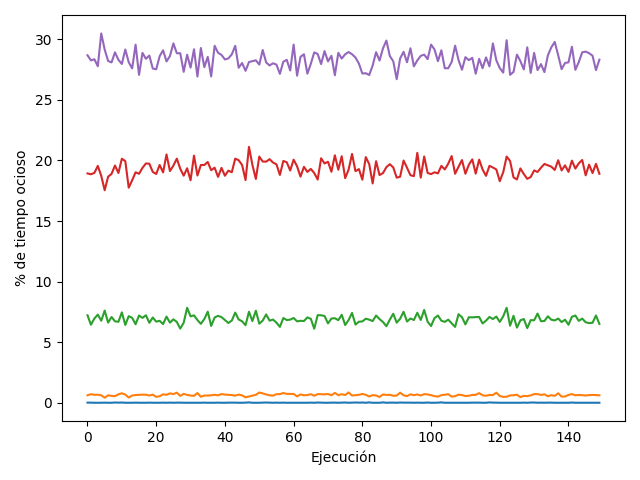
\includegraphics[scale=0.4]{img/incremento-fijo-ocioso.png}
\end{minipage}%
\begin{minipage}{0.5\textwidth}
  \centering
  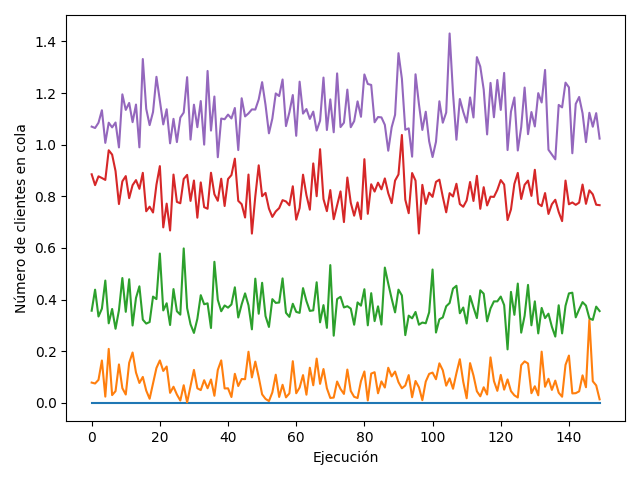
\includegraphics[scale=0.4]{img/incremento-fijo-cola.png}
\end{minipage}
\caption{Porcentaje de tiempo ocioso del servidor y media de clientes en cola}
\end{figure}

Aqui podemos observa cómo las gráficas van teniendo un porcentaje de ocupación y un número de clientes en cola más alto a medida que disminuimos las valores $tlleg$
y $tserv$. También podemos observar que, pese a que cada una de las líneas rondan un rango de valores, existe cierta variabilidad en los resultados; por lo cual sería
un poco irresponsable fiarnos de un solo dato como el de la tabla.


\section{Simulación con incremento variable de tiempo}

Ahora vamos a tratar el mismo problema pero con un incremento de tiempo variable, para hacerlo más eficiente y preciso. En este caso, la variable no tendrá ni por
qué ser un entero ni tendremos que parsear los generadores de datos, ya que se incrementará su valor hasta el suceso más cercano. Decimos que es más preciso porque
porque no tiene que dar los saltos que daba el anterior modelo y, en consecuencia, gana en eficiencia ya que va suceso a suceso.

Esta es la nueva línea de código que tendremos que añadir (también quitaremos la que aumenta el tiempo de manera uniforme $reloj++$):
\begin{lstlisting}
reloj = min(tiempo_llegada,tiempo_salida)
\end{lstlisting}

A continuación, vamos a ejecutar este modelo de la misma forma que hemos hecho con el modelo anterior y óbservar los cambios que se obtienen:

\begin{table}[H]
\resizebox{\textwidth}{!}{%
\begin{tabular}{c|c|c|c|c}
\textbf{tiempo} & \textbf{tlleg} & \textbf{tserv} & \textbf{\% tiempo ocioso} & \textbf{Media clientes en cola} \\ \hline
horas           & 0.15           & 0.1            & 33.993752                 & 1.260754                        \\ \hline
medias horas    & 0.3            & 0.2            & 33.555038                 & 1.250663                        \\ \hline
cuartos de hora & 0.6            & 0.4            & 34.353592                 & 1.382941                        \\ \hline
minutos         & 9              & 6              & 34.451107                 & 1.211860                        \\ \hline
segundos        & 540            & 360            & 33.695103                 & 1.261086                        \\
\end{tabular}%
}
\end{table}

Vemos que los resultados esta vez han sido más regulares, ya que para todas las medidas de tiempo se han obtenido unos valores entre el 33 y el 34 por ciento. A
diferencia del modelo anterior, en este podríamos decir que los resultados son bastante más fiables independientemente de si utilizamos horas, minutos, segundos...
Esto es debido a que ahora no tenemos la acumulación del error que teníamos anteriormente, y los sucesos se producen siempre en el momento declarado, sin ponderar.
\begin{figure}[H]
\centering
\begin{minipage}{0.5\textwidth}
  \centering
  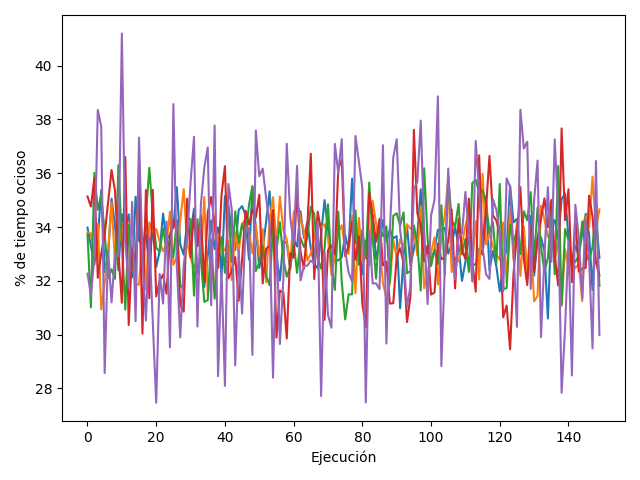
\includegraphics[scale=0.4]{img/incremento-variable-ocioso.png}
\end{minipage}%
\begin{minipage}{0.5\textwidth}
  \centering
  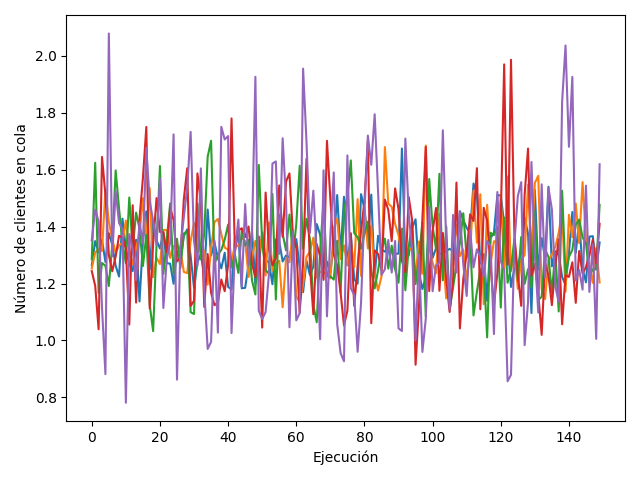
\includegraphics[scale=0.4]{img/incremento-variable-cola.png}
\end{minipage}
\caption{Porcentaje de tiempo ocioso del servidor y media de clientes en cola}
\end{figure}

Si observamos ahora las gráficas con las diversas ejecuciones, vemos que están prácticamente todas unas encima de otras. Como acabamos de decir, ya no tenemos este
error en las distintas medidas de tiempo. No obstante, vemos que aún tenemos bastante variabilidad en los datos, llegando algunos a máximos como 42 o a mínimos
como 27.

Por otra parte, esta mejora no sólo afecta a las medidas de tiempo, si no que también afecta a la eficiencia. En el modelo anterior, los incrementos en el reloj
dependen de la medida del tiempo; mientras que en el modelo actual, el número de incrementos dependerá del número de sucesos. Vamos a comprobarlo extrayendo una
tabla que compare los tiempos de ejecución para todas las medidas con incremento fijo, con las mismas medidas en incremento variable:
\begin{table}[H]
\resizebox{\textwidth}{!}{%
\begin{tabular}{c|c|c|c|c}
\textbf{tiempo} & \textbf{tlleg} & \textbf{tserv} & \textbf{tiempo fijo} & \textbf{tiempo variable} \\ \hline
horas           & 0.15           & 0.1            & 0.001671             & 0.002071                 \\ \hline
medias horas    & 0.3            & 0.2            & 0.002937             & 0.002562                 \\ \hline
cuartos de hora & 0.6            & 0.4            & 0.003491             & 0.001119                 \\ \hline
minutos         & 9              & 6              & 0.003358             & 0.001464                 \\ \hline
segundos        & 540            & 360            & 0.020543             & 0.002939                 \\
\end{tabular}%
}
\end{table}

Podemos ver que el tiempo de ejecución en el modelo con incremento fijo va aumentando lo que parece lineal o exponencialemente, mientras que en el modelo con
incremento variable tenemos unos tiempos prácticamente iguales en unas ejecuciones y otras.

\begin{figure}[H]
\centering
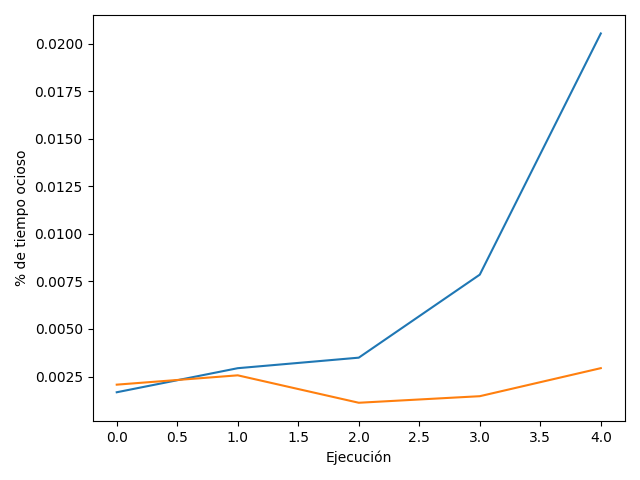
\includegraphics[scale=0.7]{img/tiempos.png}
\caption{En azul los tiempos con incremento fijo y, en naranja, variable.}
\end{figure}

En la gráfica lo podemos corroborar. Tras estudiar los dos modelos, concluímos que utilizar uno de incremento variable sería lo acertado, no sólo por la mayor
eficiencia en tiempo que nos da, si no por algo más importante como es la precisión y calidad al trabajar con distintos tipos de datos o unidades de medida.




\section{Programa de simulación dinámico y discreto}

En esta sección vamos a abordar un problema similar al anterior, pero con una cantidad de $m$ servidores idénticos trabajando en paralelo. La cola de clientes
seguirá siendo la misma, tratando a los clientes del mismo método FIFO. Si utilizamos más de un servidor en complicado, pero con $m=1$ es posible obtener los
valores teóricos de casi todas las medidas de rendimiento.

Vamos a ejecutar el programa para ver qué resultamos obtenemos. Lo haremos con unos parámetros como los anteriores ($parada=10.000$, $tlleg=9$ y $tserv=6$):
\begin{figure}[H]
\centering
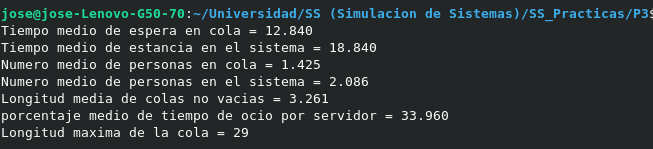
\includegraphics[scale=0.8]{img/cola-m1.png}
\caption{Ejecución del programa colammk con $m=1$.}
\end{figure}

Una vez obtenidos estos valores, vamos a contrastarlos con los teóricos. Lo primero es calcularlos:

\begin{itemize}[label=\textbullet]
	\item Tiempo medio de espera en cola
		  $= \frac{tserv^2}{tlleg-tserv} = \frac{6^2}{9-6} = \frac{36}{3} = 12$
	\item Tiempo medio de estancia en el sistema
		  $= \frac{tserv \cdot tlleg}{tlleg-tserv} = \frac{6 \cdot 9}{9-6} = \frac{54}{3} = 18$
	\item Número medio de clientes en cola
		  $= \frac{tserv^2}{tlleg (tlleg-tserv)} = \frac{6^2}{9\cdot (9-6)} = \frac{36}{27} = 1.3$
	\item Número medio de clientes en el sistema
		  $= \frac{tserv}{tlleg-tserv} = \frac{6}{9-6} = \frac{6}{3} = 2$
	\item Longitud media de colas no vacías
		  $= \frac{tlleg}{tlleg-tserv} = \frac{9}{9-6} = \frac{9}{3} = 3$
	\item Porcentaje de tiempo de ocio del servidor
		  $= \big(1 - \frac{tserv}{tlleg}\big) \cdot 100 = \big(1 - \frac{6}{9}\big) \cdot 100 = \frac{100}{3} = 33.3$
\end{itemize}

Como podemos ver, los resultados se ajustan bastante bien a los que esperábamos teóricamente. Esto se debe, en parte, a que la simulación se ha realizado con
un tiempo de parada muy alto, es decir, la simulación ha durado bastante tiempo y las medias que se obtienen son lo suficientemente representativas.

Si probamos con un tiempo de parada bajo, los resultados serán más impredecibles o variables, como se muestra a continuación:
\begin{figure}[H]
\centering
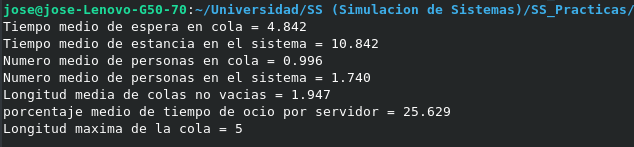
\includegraphics[scale=0.8]{img/cola2-m1.png}
\caption{Ejecución del programa colammk con $m=1$ y tiempo bajo.}
\end{figure}


Ahora vamos a aumentar el número de servidores $m$, pero manteniendo un equilibrio. El tiempo de servicio dividido por el número de servidores tiene que
permanecer constante. Vamos a modificar el programa para que repita varias veces la simulación y calcule las medias y desviaciones típicas de las medidas
de rendimiento.

Las líneas más importantes que se han modificadas son las siguientes:
\begin{lstlisting}
void fin(){
	....
	// Variables nuevas para medias y desviaciones
	retrasoMedio += retrasomedio;
	estanciaMedia += estanciamedia;
	enColaMedio += encolamedio;
	enSistemaMedia += ensistemamedio;
	colasMedia += colasnovaciasmedio;
	porcentajeOcioMedio += porcentajemedioocio;
	longMaxCola += maximacola;

	retrasoMedioDes += pow(retrasomedio, 2);
	estanciaMediaDes += pow(estanciamedia, 2);
	enColaMedioDes += pow(encolamedio, 2);
	enSistemaMedioDes += pow(ensistemamedio, 2);
	colasMediaDes += pow(colasnovaciasmedio, 2);
	porcentajeOcioMedioDes += pow(porcentajemedioocio, 2);
	longMaxColaDes += pow(maximacola, 2);
}
\end{lstlisting}
\begin{lstlisting}
float calcularDesviacion(float suma, float media)
{
    float desviacion = suma - (n_simulaciones * pow(media, 2));
    desviacion = desviacion / (n_simulaciones - 1);

    return sqrt(desviacion);
}
\end{lstlisting}

Por último ya tenemos el bucle for, la división entre el número de simulaciones para hacer la media y desviaciones típicas, y posteriormente imprimimos
los resultados.

La prueba de este programa la vamos a realizar con varios números de servidores, sin embargo, el resto de parámetros que usaremos serán los mismos que
los de la ejecución con $m=1$, ya que los resultados obtenidos eran muy similares a los valores teóricos. En este caso vamos a realizar la ejecución con
2, 3, 4 y 5 servidores, adaptando el $tserv$ a cada uno de ellos para mantener el equilibrio. Este ha sido el resultado:

\begin{table}[H]
\centering
\resizebox{\textwidth}{!}{%
\begin{tabular}{c|c|c|c|c}
\textbf{\begin{tabular}[c]{@{}c@{}}Número de\\ servidores\end{tabular}} & \textbf{\begin{tabular}[c]{@{}c@{}}2\\ tserv: 12\end{tabular}} & \textbf{\begin{tabular}[c]{@{}c@{}}3\\ tserv: 18\end{tabular}} & \textbf{\begin{tabular}[c]{@{}c@{}}4\\ tserv: 24\end{tabular}} & \textbf{\begin{tabular}[c]{@{}c@{}}5\\ tserv: 30\end{tabular}} \\ \hline
\textbf{\begin{tabular}[c]{@{}c@{}}Tiempo medio\\ espera en cola\end{tabular}} & \begin{tabular}[c]{@{}c@{}}med: 9.41335\\ des: 0.730856\end{tabular} & \begin{tabular}[c]{@{}c@{}}med: 7.80226\\ des: 1.19625\end{tabular} & \begin{tabular}[c]{@{}c@{}}med: 6.5818\\ des: 1.59282\end{tabular} & \begin{tabular}[c]{@{}c@{}}med: 5.78543\\ des: 0.709112\end{tabular} \\ \hline
\textbf{\begin{tabular}[c]{@{}c@{}}Tiempo medio\\ estancia en el sistema\end{tabular}} & \begin{tabular}[c]{@{}c@{}}med: 21.4133\\ des: 0.730836\end{tabular} & \begin{tabular}[c]{@{}c@{}}med: 25.8023\\ des: 1.19633\end{tabular} & \begin{tabular}[c]{@{}c@{}}med: 30.5818\\ des: 1.59289\end{tabular} & \begin{tabular}[c]{@{}c@{}}med: 35.7854\\ des: 0.70908\end{tabular} \\ \hline
\textbf{\begin{tabular}[c]{@{}c@{}}Numero medio\\ personas en cola\end{tabular}} & \begin{tabular}[c]{@{}c@{}}med: 1.05059\\ des: 0.0854933\end{tabular} & \begin{tabular}[c]{@{}c@{}}med: 0.883231\\ des: 0.0896291\end{tabular} & \begin{tabular}[c]{@{}c@{}}med: 0.746949\\ des: 0.0693109\end{tabular} & \begin{tabular}[c]{@{}c@{}}med: 0.649897\\ des: 0.0780725\end{tabular} \\ \hline
\textbf{\begin{tabular}[c]{@{}c@{}}Número medio\\ personas en el sistema\end{tabular}} & \begin{tabular}[c]{@{}c@{}}med: 2.37887\\ des: 0.0963648\end{tabular} & \begin{tabular}[c]{@{}c@{}}med: 2.87863\\ des: 0.103085\end{tabular} & \begin{tabular}[c]{@{}c@{}}med: 3.40728\\ des: 0.0925651\end{tabular} & \begin{tabular}[c]{@{}c@{}}med: 3.98036\\ des: 0.118443\end{tabular} \\ \hline
\textbf{\begin{tabular}[c]{@{}c@{}}Longitud media\\ colas no vacías\end{tabular}} & \begin{tabular}[c]{@{}c@{}}med: 2.97911\\ des: 0.172741\end{tabular} & \begin{tabular}[c]{@{}c@{}}med: 2.99961\\ des: 0.209258\end{tabular} & \begin{tabular}[c]{@{}c@{}}med: 2.98825\\ des: 0.184951\end{tabular} & \begin{tabular}[c]{@{}c@{}}med: 2.97684\\ des: 0.214132\end{tabular} \\ \hline
\textbf{\begin{tabular}[c]{@{}c@{}}Porcentaje medio\\ tiempo de ocio\end{tabular}} & \begin{tabular}[c]{@{}c@{}}med: 33.5856\\ des: 0.744918\end{tabular} & \begin{tabular}[c]{@{}c@{}}med: 33.4867\\ des: 0.718379\end{tabular} & \begin{tabular}[c]{@{}c@{}}med: 33.4917\\ des: 0.822586\end{tabular} & \begin{tabular}[c]{@{}c@{}}med: 33.3909\\ des: 1.01696\end{tabular} \\ \hline
\textbf{\begin{tabular}[c]{@{}c@{}}Longitud\\ máxima cola\end{tabular}} & \begin{tabular}[c]{@{}c@{}}med: 18.4\\ des: 3.43452\end{tabular} & \begin{tabular}[c]{@{}c@{}}med: 17.88\\ des: 3.86317\end{tabular} & \begin{tabular}[c]{@{}c@{}}med: 17.16\\ des: 3.32191\end{tabular} & \begin{tabular}[c]{@{}c@{}}med: 16.5\\ des: 2.74234\end{tabular}
\end{tabular}%
}
\end{table}

Podemos ver que a medida que aumentamos el número de servidores, los resultados van siendo mejores. Los tiempos medios de espera en cola se reducen, con
menos clientes en cola y, a su vez, un número mayor de clientes en el sistema.

Por otro lado, podemos ver que el porcentaje medio de tiempo de ocio del servidor es prácticamente el mismo en todos los casos (teniendo en cuenta siempre
un cierto error) y el tiempo medio de estancia en el sistema se va incrementando. Esto quiere decir que el sistema está bien equilibrado y, a su vez, deducimos
que estamos desperdiciando potencia del servidor; es decir, que pese a tener un número alto de servidores, no tenemos los suficientes clientes para que funcionen
eficientemente o, simplemente, no los distribuímos de una forma eficaz.

\newpage
Para finalizar con este modelo de simulación, vamos a estudiar que sucede si reemplzamos los generadores actuales por generadores determinísticos y uniformes.
El nuevo código implementado para el determinístico y para el uniforme, respectivamente, es:
\begin{lstlisting}
// Deterministico. Devuelve siempre el valor medio introducido
float generador_deterministico(float media)
{
	return media;
}

// Uniforme. Devuelve un valor uniformemente generado con media
// en el valor introducido
float generador_uniforme(float media)
{
	float u;
	u = (float) random();
	u = u/(float)(RAND_MAX+1.0);
	return(media*2*u);
}
\end{lstlisting}

Las pruebas también se van a hacer con una cantidad $m=1$ de servidores y con el resto de parámetros igual que en las pruebas anteriors. El resultado es el
siguiente:
\begin{table}[H]
\centering
\begin{tabular}{c|c|c}
\textbf{\begin{tabular}[c]{@{}c@{}}Tipo de\\ generador\end{tabular}} & \textbf{\begin{tabular}[c]{@{}c@{}}Generador\\ determinístico\end{tabular}} & \textbf{\begin{tabular}[c]{@{}c@{}}Generador\\ uniforme\end{tabular}} \\ \hline
\textbf{\begin{tabular}[c]{@{}c@{}}Tiempo medio\\ espera en cola\end{tabular}} & 0 & 3.498 \\ \hline
\textbf{\begin{tabular}[c]{@{}c@{}}Tiempo medio\\ estancia en el sistema\end{tabular}} & 6 & 9.498 \\ \hline
\textbf{\begin{tabular}[c]{@{}c@{}}Numero medio\\ personas en cola\end{tabular}} & 0 & 0.387 \\ \hline
\textbf{\begin{tabular}[c]{@{}c@{}}Número medio\\ personas en el sistema\end{tabular}} & 0.667 & 1.051 \\ \hline
\textbf{\begin{tabular}[c]{@{}c@{}}Longitud media\\ colas no vacías\end{tabular}} & 0 & 1.519 \\ \hline
\textbf{\begin{tabular}[c]{@{}c@{}}Porcentaje medio\\ tiempo de ocio\end{tabular}} & 33.339 & 33.534 \\ \hline
\textbf{\begin{tabular}[c]{@{}c@{}}Longitud\\ máxima cola\end{tabular}} & 0 & 6
\end{tabular}
\end{table}

Como podemos ver, el generador determinístico ha obtenido los mejores resultados posibles, con un tiempo medio de espera en la cola de 0 minutos y un tiempo
de servicio medio de 6 minutos. Esto se debe a que el generador de tiempos de servicio no produce las variaciones que se pueden dar en la vida real, y por lo
tanto, como el tiempo de llegadas es 9 minutos y el de servicio 6, nunca se pisrán el uno con el otro.

En cuanto al generador uniforme, vemos que nos da resultados diferentes a los del generador determinístico y que, en un principio, parecen bastante buenos. No
obstante, si los comparamos con los valores teóricos calculados anteriormente, vemos que son muy diferentes, lo que quiere decir que son unos valores bastante
alejados de la realidad.




\chapter{Mi tercer modelo de simulación Discreto}

\section{Remolcador de un puerto}


\section{Mejoras propuestas para el remolcador}




\chapter{Análisis de Salidas y Experimentación}

\section{¿Cuánto hay que simular?}

\section{Intervalos de confianza}

\section{Comparación de más de dos sistemas}

\end{document}



